
\chapter{  Analyse des besoins et conception}
%\tableofcontents

\textbf{\huge Introduction}\\[0.5cm] 

L'objectif de l'étape de spécification et d'analyse des besoins est de déterminer les fonctionnalités différentes attendues du système. Au cours de ce chapitre, nous présentons d'abord les acteurs concernés dans notre système. Ensuite, nous allons illustrer les besoins fonctionnels et non fonctionnels. Puis, nous allons détailler le product backlog de notre projet. Ces exigences seront exprimées enfin sous forme de diagramme de cas d'utilisation qui sera détaillé par des scénarios possibles.Par la suite,nous présentons la conception de notre application qui présente une étape fondamentale qui précède la réalisation par une description des différents diagrammes de séquence, classe et déploiement. Nous procédons ensuite à la définition de la méthodologie de conception. Et nous terminons par représenter l'architecture technique de notre projet.
\section{\LARGE Acteurs}
\texttt{}\\[0.1cm]
 En génie logiciel et plus particulièrement en UML, un acteur est une entité qui définit le rôle joué par un utilisateur ou par un système qui interagit avec le système modélisé\cite{12}.\\\texttt{}\\[0.01cm]%add url
 \textsf{\fontfamily{ptm}\selectfont\scalefont{1.3}--Développeur :}C'est l'utilisateur qui peut modifier le code source d'un objectif donné (ajouter une fonctionnalité, corriger l'erreur, etc.) puis les déposer dans Github et ensuite suivre la compilation de l'application.\\\texttt{}\\[0.01cm]
\textsf{\fontfamily{ptm}\selectfont\scalefont{1.3}-- Ingénieur DevOps:} Est considéré comme l'acteur principal, son rôle est la mise en place du cluster, pipeline, surveiller l'état du système et configurer son infrastructure.\\\texttt{}\\[0.01cm]
\textsf{\fontfamily{ptm}\selectfont\scalefont{1.3}-- Client:} C'est l'utilisateur qui peut accéder à l'application déployée sur le cluster au moyen d'un site Web.\\\texttt{}\\[0.01cm]


\section{\LARGE Besoins fonctionnels}
\texttt{}\\[0.1cm]
 Pour le bon fonctionnement de notre projet, il est nécessaire de définir  concrètement les fonctionnalités qui seront implémentées dans le but de les rendre plus appropriées aux besoins de l'entreprise.
Pour cela nous avons allons présenter les besoins fonctionnels de notre projet:\\\texttt{}\\[0.01cm]
-- Mettre en place une solution hybride qui permet à l'entreprise d'exécuter des applications localement tout en profitant des avantages des services cloud.\\\texttt{}\\[0.01cm]
– Orchestrer les conteneurs pour garantir une haute disponibilité pour le déploiement et l'exécution des applications.\\\texttt{}\\[0.01cm]
– Automatiser le processus de déploiement avec Ansible pour aider avec les charges de travail.\\\texttt{}\\[0.01cm]
– Surveiller l’état du déploiement.\\\texttt{}\\[0.01cm]
– Créer un répertoire pour toutes les images Docker dans ECR (Elastic Container Registry).\\\texttt{}\\[0.01cm]
-- Enregistrer les artefacts dans un répertoire Nexus.\\\texttt{}\\[0.01cm]
– Utiliser Prometheus et Grafana pour surveiller le cluster kubernetes.\\\texttt{}\\[0.01cm]
– Assurer la qualité de code source avec SonarQube.\\\texttt{}\\[0.01cm]
– Gérer automatique des étapes de déploiement de clusters.


\section{\LARGE Besoins non-fonctionnels}
\texttt{}\\[0.1cm]
 Les besoins non fonctionnels établissent toutes les conditions nécessaires au bon fonctionnement du système et à l'amélioration de la qualité des services. Et pour répondre aux exigences fonctionnelles, notre projet doit respecter une série de propriétés contribuant à une meilleure qualité de la solution obtenue.
Nous déterminerons l'ensemble des contraintes à respecter pour garantir le bon déroulement du projet. Parmi les critères nous citons :\\\texttt{}\\[0.01cm]
--Confidentialité: Notre solution permettra de garantir la sécurité des données, des applications et des utilisateurs.\\\texttt{}\\[0.01cm]
--Performance: Rapidité du déploiement d'application sur des pods kubernetes et assurer la bonne exécution de ses applications.\\texttt{}\\[0.01cm]
--Disponibilité: Les clusters Kubernetes sont conçus pour permettre une évolutivité horizontale, ce qui signifie que les applications peuvent être déployées sur plusieurs nœuds et gérer de manière dynamique les charges de travail en fonction des besoins.\\\texttt{}\\[0.01cm]
--Maintenance: La modification d'un déploiement dans un kubernetes cluster doit être facilement maintenable et adaptable à de nouvelles exigences de sorte qu'il peut y avoir un changement ou l'ajout de nouvelle fonctionnalité.\\\texttt{}\\[0.01cm]
--Portabilité: Le système doit être flexible et capable de prendre en charge de nouvelles fonctions et extensions et doit pouvoir fonctionner avec un nouveau composant (RAM,stockage) et avec une modification minimale.\\\texttt{}\\[0.01cm]
--Extensibilité: Le système doit maintenir ses hautes performances sous pression et ajuster ses paramètres pour répondre à la demande, possibilité d’ajouter des nœuds en cas de montée en charge. \\\texttt{}\\[0.01cm]

\section{\LARGE Product Backlog}

Product Backlog est une liste de toutes les tâches connues pour être traitées par le produit. Il s'agit de la seule source des besoins pour toute modification du produit. Les besoins sont précisés par les user stories. Un "user story" se présente sous la forme suivante (voir tableau 2.1): \\[0.1cm]

\begin{table}[H]
  \begin{center}
    \resizebox{1.1\textwidth}{!}{%
  \begin{tabular}{|c|c|c| p{5cm}|c|}
    \hline
    id & Theme & Acteur & Description & Priorité \\
    \hline
    id 1 & gérer code source & Développeur & Permet de déposer le code ou le récupérer  & élevée \\
    \hline
    id2 & Suivre build d'application & Développeur & Peut voir la compilation de l'application & élevée \\
    \hline
    id3 & analyser qualité de code & Ingénieur DEVOPS & Permet  d'analyser le code source d'un projet et de détecter les erreurs de qualité avec SonarQube . &  élevée \\
    \hline
    id 4  & gérer liste des images docker & Ingénieur DEVOPS &  Consiste à répertorier et organiser les images Docker qui ont été créées .&  élevée \\
    \hline
    id 5 & gérer les artefacts d'application & Ingénieur DEVOPS &  Consiste à stocker et à gérer les différents composants d'une application, les bibliothèques, les configurations, les scripts et autres ressources .&  élevée \\
    \hline
    id 6 & Configurer l'architecture cloud & Ingénieur DEVOPS & Consiste à concevoir et à déployer une infrastructure informatique dans le cloud, en utilisant des services cloud pour répondre aux besoins. &  élevée \\
    \hline
    id 7 & Configurer le pipline & Ingénieur DEVOPS &  Est un processus important pour automatiser le processus de développement, de test et de déploiement d'une application. &  élevée \\
    \hline
    id 8  & Surveiller l'etat du cluster & Ingénieur DEVOPS &  Surveille l'état de tous les nœuds dans le cluster pour s'assurer qu'ils sont en bon état de fonctionnement et qu'ils répondent aux demandes des applications. &  élevée \\
    \hline
    id 9 & gérer la configuration du deploiement & Ingénieur DEVOPS & Assure que les applications sont déployées de manière cohérente et fiable &  élevée \\
    \hline
    id 10 & acces a l'application deployée & Client & s'assure qu'elle est accessible uniquement par les utilisateurs autorisés. &  élevée \\
    \hline
  \end{tabular}%
    }
  \end{center}
  \caption{Tableau du Product Back-log}
  \end{table}
  \texttt{}\\[0.5cm]

%\section{\LARGE  Conception de système}
%\textsf{\fontfamily{qtm}\selectfont\scalefont{1.3}
%Dnas ce qui suit,nous allons présenter les différent diagrammes de conception. }//[0.2cm]
\section{\Large  Diagramme de cas d'utilisation Global}


Le diagramme de cas d'utilisation global est utilisé pour une représentation du comportement fonctionnel d'un système logiciel.\\\texttt{}\\[0.01cm]
Le diagramme ci-dessous présente les cas d'utilisation généraux et les acteurs qui interagissent avec le système(Voir figure 2.1).
\begin{figure}[H]
  \begin{center}
  
      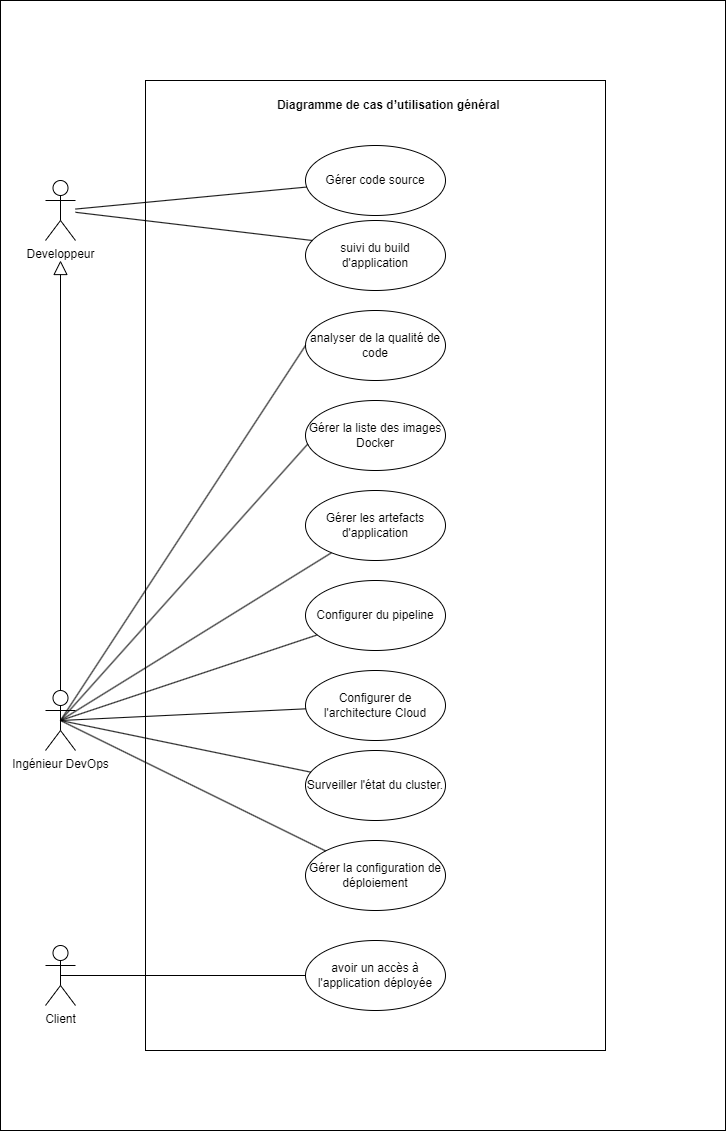
\includegraphics[width=12cm]{Use case.drawio.png}

  \end{center}
  
  \caption{Diagramme de cas d'utilisation Globale}
\end{figure}


Dans ce qui suit , le raffinnement des différents cas d'utilisation.\\[0.2cm]
\subsection{\Large Cas d’utilisation "Gérer code source"}
Dans cette section, nous décrirons de façon détaillée ce cas d'utilisation.\\\texttt{}\\[0.01cm]

\begin{figure}[H]
  \begin{center}
  
      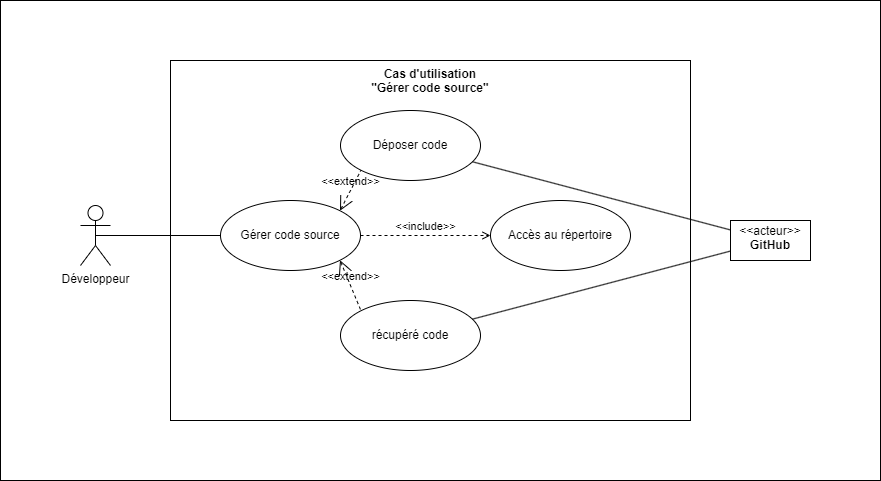
\includegraphics[width=15cm]{usecase1.drawio.png}

  \end{center}
  
  \caption{Cas d'utilisation:Gérer code source }
\end{figure}

Pour expliquer  le diagramme de cas d’utilisation, nous représentons la description textuelle du principales fonctionnalités mentionnées ci-dessus (Voir tableau 2.2): \\

\begin{center}
 \begin{table}[H] 
 \centering
 \resizebox{1.1\textwidth}{!}{%
 \begin{tabular}{|c|p{13cm}|}
 \hline
 Titre & Gérer code source\\
 \hline
 Acteur & Développeur \\
 \hline
 Description & le développeur peut déposer ou récupérer le code à travers le command "pull" ou "push".\\
 \hline
 Pré conditions & Une connexion établie entre le PC du développeur et le répertoire Git de l'application. \\
 \hline
 Post conditions & Code envoyé au répertoire git. \\
 \hline 
 \multirow{3}{*}{Scénario nominal} & 1- Avoir un accès au répertoire. \\
 & 2 - Gérer code source. \\
 & 3 - Déposer ou récuperer  le code dans le répertoire github. \\
 \hline
 \multirow{3}{*}{Scénario alternatif} & 1- La connexion entre la machine du développeur et Git ne peut pas être établie. \\
 & 2 - Le code ne peut pas être envoyé. \\
 & 3 - Retour à l'étape 1 du Scénario nominal. \\ 
 \hline
 \end{tabular}%
 }
 \caption{Description de cas d’utilisation:Gérer code source}
 \end{table}
\end{center}


   \subsection{\Large Cas d’utilisation "Suivi de la build d'application"}

Dans cette section, nous décrirons de façon détaillée ce cas d'utilisation.\\\texttt{}\\[0.01cm]

\begin{figure}[H]
  \begin{center}
  
      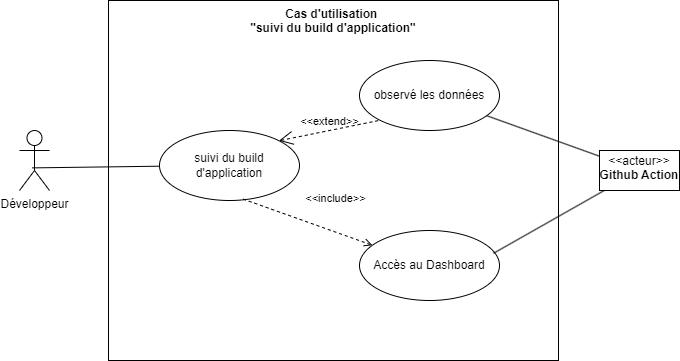
\includegraphics[width=15cm]{UseCase2.drawio.png}

  \end{center}
  
  \caption{Cas d'utilisation:Suivi la build d'application }
\end{figure}

Pour expliquer  le diagramme de cas d’utilisation, nous représentons la description textuelle des principales fonctionnalités mentionnées ci-dessus(voir tableau 2.3 ) : \\
\begin{center}
   \begin{table}[H]  
     \centering
     \resizebox{1.1\textwidth}{!}{%
     \begin{tabular}{|c|p{13cm}|}
      \hline
      Titre &  Suivi du build de l'application\\
      \hline
      Acteur & Développeur \\
      \hline
      Description & Le développeur peut suive la construction d'application pour connaître si la modification ajoutée au code source est valide ou non.\\
      \hline
      Pré conditions & Une connexion  établie entre le développeur et Github actions. \\
      \hline
      Post conditions & Affichage de Dashboard Github Actions. \\
      \hline 
      \multirow{3}{*}{Scénario nominal} & 1- Avoir un accès au Dashbord \\ 
      & 2- Suivi du build de l'application \\
      & 3- L'observation de la construction de l'application rapporte un succès.\\
      \hline
      \multirow{2}{*}{Scénario alternatif} & 1 - La connexion entre développeur et Github Actions ne peut pas être établie. \\
      & 2 - Retour à l'étape 1 du Scénario nominal.\\ 
      \hline
      \end{tabular}%
     }
   \caption{Description de cas d’utilisation:Suivi du build de l'application}
   \end{table}
   \end{center}
   \subsection{\Large Cas d'utilisation"Gérer la configuration de déploiement"}
    Dans cette section, nous décrirons de façon détaillée ce cas d'utilisation(voir figure 2.4).\\\texttt{}\\[0.01cm]
   
   \begin{figure}[H]
    \begin{center}
    
        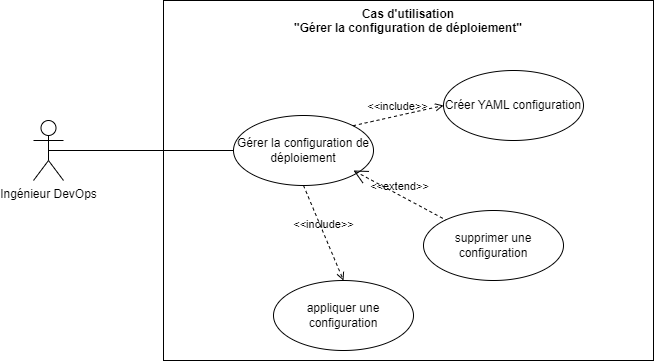
\includegraphics[width=15cm]{UserCase3.drawio.png}
  
    \end{center}
    
    \caption{Cas d'utilisation:Gérer la configuration de déploiement}
  \end{figure}
   
   Pour expliquer  le diagramme de cas d’utilisation, nous représentons la description textuelle des principales fonctionnalités mentionnées ci-dessus (voir table 2.4)  : \\
   \begin{center}
      \begin{table}[H]  
        \centering
        \resizebox{1.1\textwidth}{!}{%
        \begin{tabular}{|c|p{13cm}|}
         \hline
         Titre & Gérer la configuration de déploiement\\
         \hline
         Acteur & Ingénieur DevOps \\
         \hline
         Description & L'ingénieur DevOps gére la configuration de déploiement pour assurer la meilleure performance du cluster.\\
         \hline
         Pré conditions & Fonctionnement correct du cluster EKS. \\
         \hline
         Post conditions & Une configuration ou modification d'une configuration déjà existante. \\
         \hline 
        \multirow{2}{*}{Scénario nominal} & 1 - Lancer la configuration  du déploiement. \\
        & 2 - La configuration est lancée dans le contrôle plane d'EKS.\\
         \hline
        \multirow{3}{*}{Scénario alternatif} & 1 - La  nouvelle configuration n'est pas flexible. \\
        & 2 - Un problème apparaît causé par la nouvelle configuration.  \\
        & 3 - Retour à l'étape 1 du Scénario nominal.\\
         \hline
         \end{tabular}%
         }
      \caption{Description de cas d’utilisation:Gérer la configuration de déploiement}
      \end{table}
      \end{center}
      \subsubsection{\Large Cas utilisation"Gérer liste des images Docker"}
       
      Dans cette section, nous décrirons de façon détaillée le cas d'utilisation (voir figure 2.5).\\\texttt{}\\[0.01cm]
      
      \begin{figure}[H]
        \begin{center}
        
            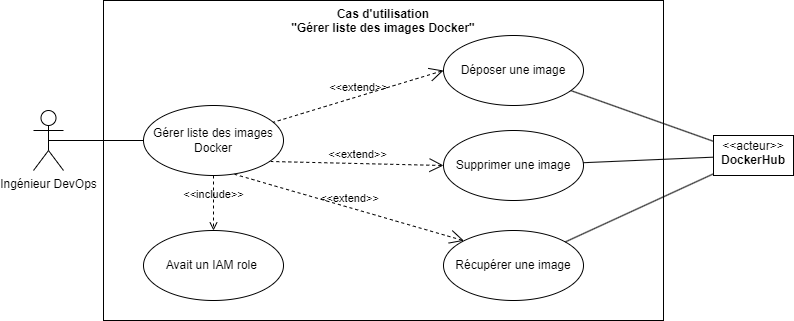
\includegraphics[width=15cm]{usecase5.drawio.png}
      
        \end{center}
        
        \caption{Cas d'utilisation:Gérer liste des images Docker}
      \end{figure}
      
      Pour expliquer  le diagramme de cas d’utilisation, nous représentons la description textuelle des principales fonctionnalités mentionnées ci-dessus (voir table 2.5) : \\
      \begin{center}
         \begin{table}[H]  
           \centering
           \resizebox{1.1\textwidth}{!}{%
           \begin{tabular}{|c|p{13cm}|}
            \hline
            Titre & Gérer liste des images Docker\\
            \hline
            Acteur & Ingénieur DevOps \\
            \hline
            Description & L'ingénieur DevOps gére la liste des images Docker\\
            \hline
            Pré conditions & Connexion au répertoire de l'application dans ECR. \\
            \hline
            Post conditions & Une image modifiée ,supprimée ou ajoutée. \\
            \hline 
           \multirow{4}{*}{Scénario nominal} & 1 - Se connecter ou l'enregistremementc de l'image n'est pas valide. \\
           & 2 -  Configurer liste des images Docker .\\
           & 2 - Déposer ou récuperer le code dans le répertoire ECR. \\
           & 3 - L'image est enregistrée dans la répertoire ECR.\\
            \hline
            \multirow{3}{*}{Scénario alternatif} & 1 - La connexion ou l'enregistrement de image n'est pas valide.  \\
            & 2 - Echec du dépose ou  récuperation l'image Docker .\\
            & 3 - Retour à l'étape 1 du Scénario nominal.\\
            \hline
            \end{tabular}%
           }
         \caption{Description de cas d’utilisation:Gérer liste des images Docker}
         \end{table}
         \end{center} 
         
      \subsection{\Large Cas utilisation"Gérer les artefacts d'application"}

         Dans cette section, nous décrirons de façon détaillée ce cas d'utilisation (voir figure 2.6).\\\texttt{}\\[0.01cm]
         
         \begin{figure}[H]
          \begin{center}
          
              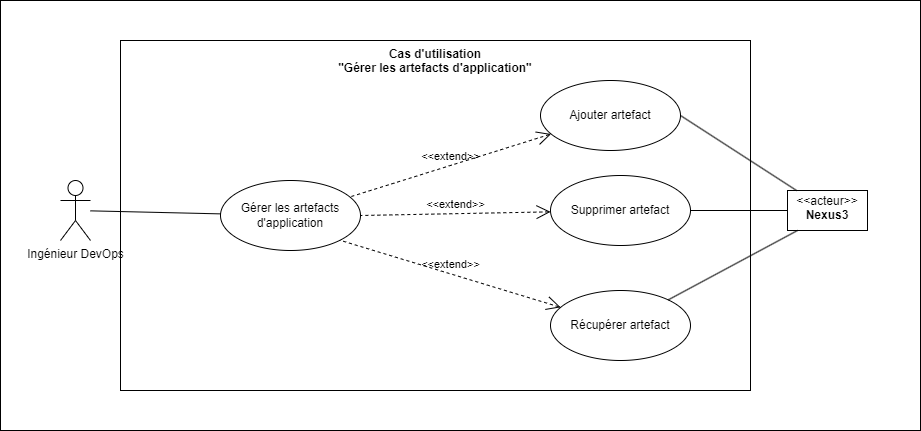
\includegraphics[width=15cm]{Usecase6.drawio.png}
        
          \end{center}
          
          \caption{Cas d'utilisation:Gérer les artefacts d'application}
        \end{figure}
         
         Pour expliquer  le diagramme de cas d’utilisation, nous représentons la description textuelle des principales fonctionnalités mentionnées ci-dessus ( voir table 2.6): \\
         \begin{center}
            \begin{table}[H]  
              \centering
              \resizebox{1.1\textwidth}{!}{%
              \begin{tabular}{|c|p{13cm}|}
               \hline
               Titre & Gérer les artefacts de l'application\\
               \hline
               Acteur & Ingénieur DevOps \\
               \hline
               Description & L'ingénieur DevOps gére la liste des artefacts pour assurer l'enregistrement de différentes versions d'application.\\
               \hline
               Pré conditions & Connexion HTTP au serveur Nexus. \\
               \hline
               Post conditions & Une répertoire avec les différentes artefacts de l'application.  \\
               \hline 
               \multirow{3}{*}{Scénario nominal} & 1 - Saisir les données d'authetification pour accéder à l'interface .\\
               & 2 - Configurer les artifacts d'application . \\
               & 3 - la connexion est réussite et la modification dans le répertoire est enregistrée dans Nexus .\\
               \hline
               \multirow{2}{*}{Scénario alternatif} & 1 - La connexion échoue ou la modification n'est pas enregistrée.  \\
               & 2 - Retour à l'étape 1 du Scénario nominal. \\
               \hline
               \end{tabular}%
              }
            \caption{Description de cas d’utilisation:Gérer les artefacts d'application}
            \end{table}
            \end{center}
  \section{\fontfamily{ptm}\selectfont\Large  Conception du système}

Dans ce qui suit,nous allons présenter les différents diagrammes de conception. \\[0.1cm]
            \subsection{\fontfamily{ptm}\selectfont\Large Diagramme de séquence global}
         Les diagrammes de séquences sont la représentation graphique des interactions entre les acteurs et le système selon un ordre chronologique\cite{14}(voir figure 3.1).
            % \begin{figure}[H]
            %   \begin{center}
            %   \centering
            %       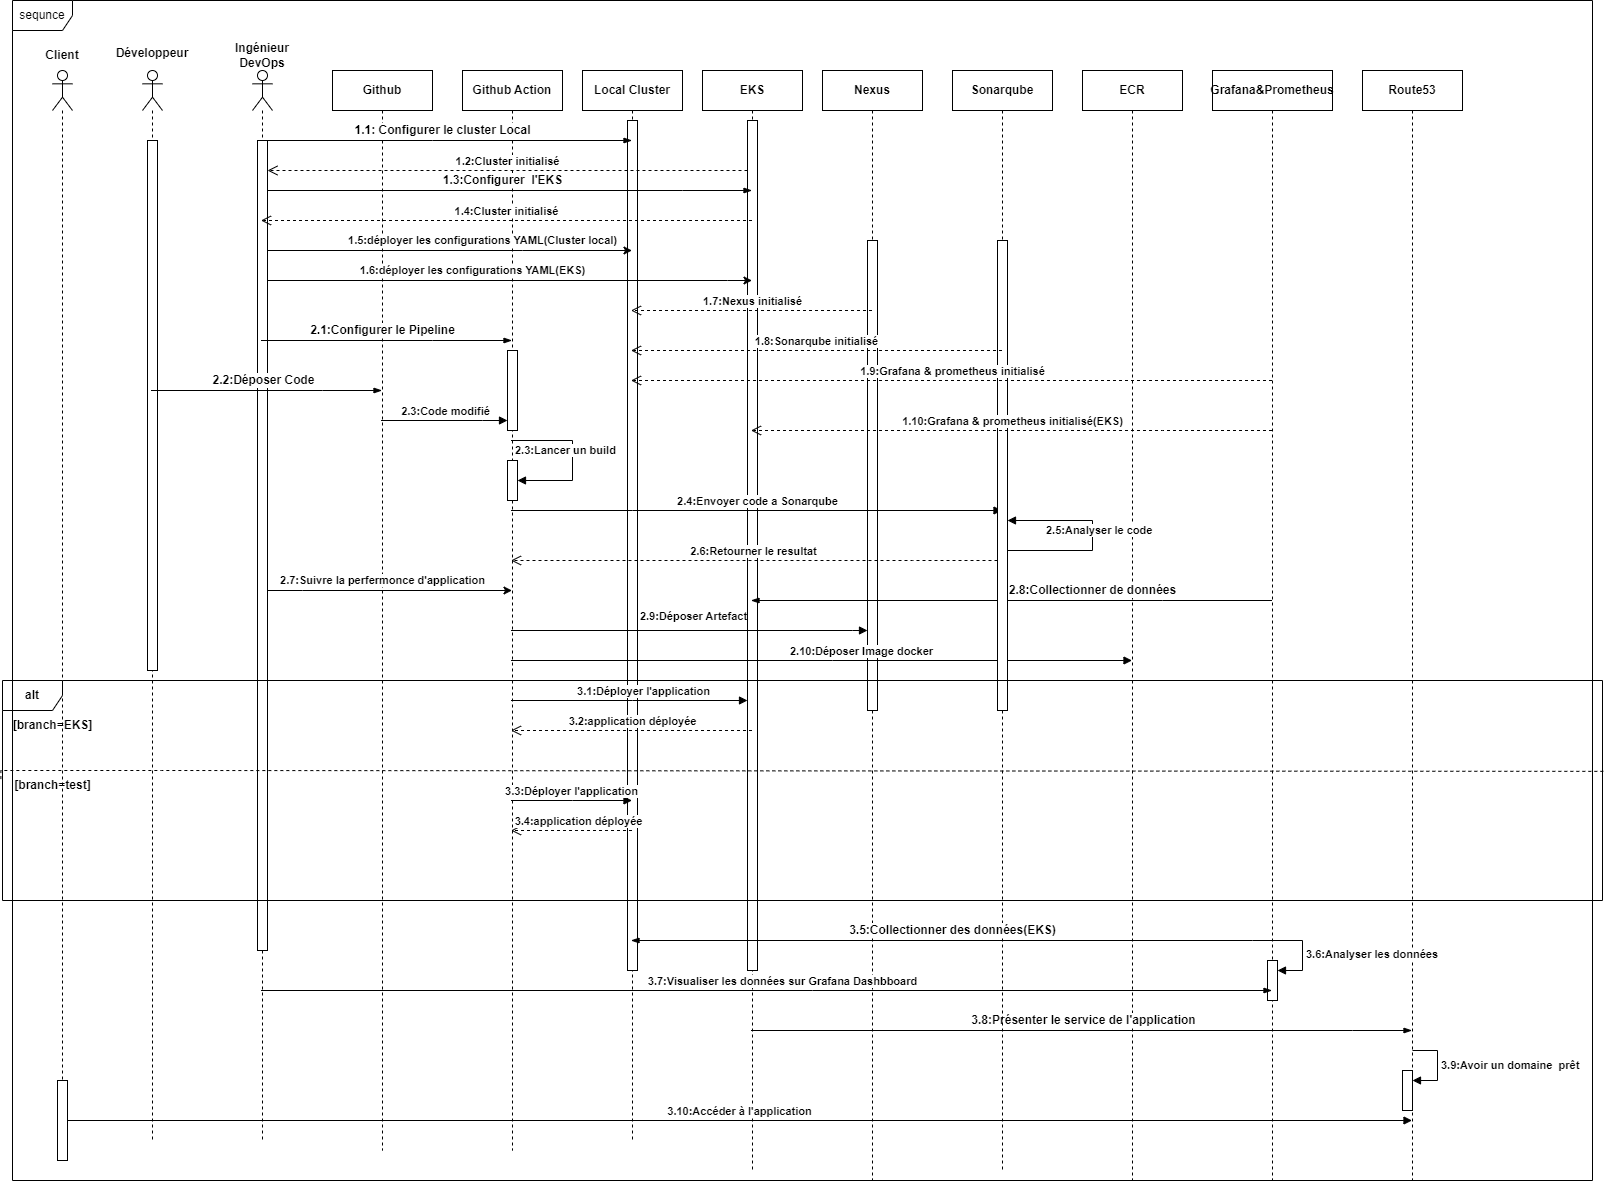
\includegraphics[height=25cm,width=18cm]{Squence.drawio.png}
            
            %   \end{center}
              
            %   \caption{Diagramme de séquence global}
            
            % \end{figure}
            \begin{landscape}
              \begin{figure}[htbp]
                \centering
                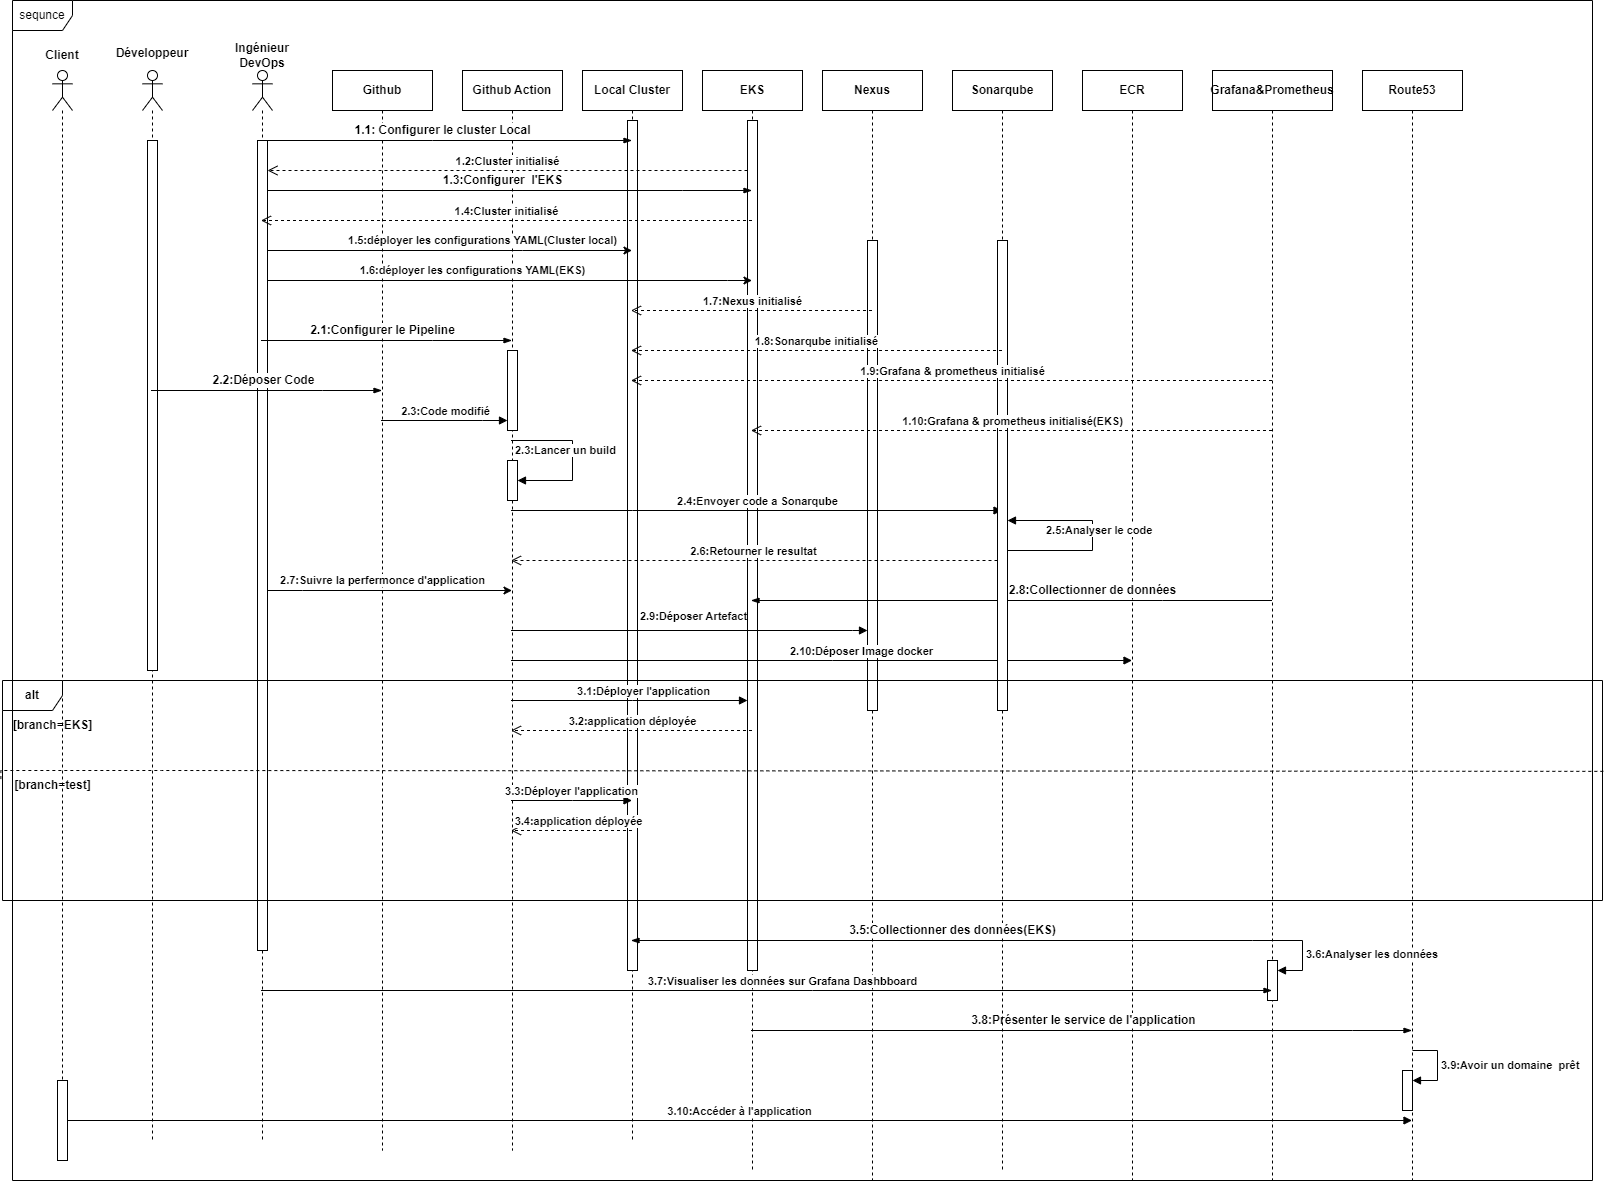
\includegraphics[width=24cm]{Squence.drawio.png} % Replace with your photo filename
                \caption{Diagramme de séquence Global}
              
              \end{figure}
            \end{landscape}
            \subsection{\fontfamily{ptm}\selectfont\Large Diagramme de séquence Détaillé}
            Pour une meilleure présentation et illustration de projet nous allons décrire les différents cas d'utilisations principaux avec leurs diagrammes de séquence détaillés.
            \subsubsection{\fontfamily{ptm}\selectfont\scalefont{1.35}Diagramme de séquence «Configuration de l'architecture cloud»}
            Nous détaillons ci-dessous les interactions du diagramme de séquence « Configuration de l'architecture cloud » 
            \begin{figure}[H]
                \begin{center}
                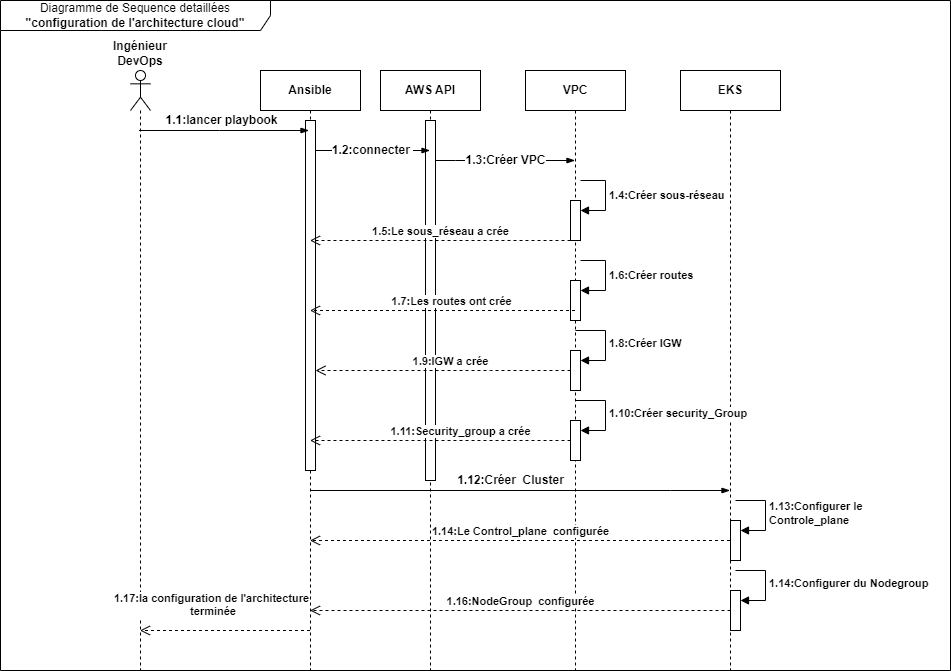
\includegraphics[height=15cm,width=18cm]{seqd.drawio.png}
                \end{center}
                \caption{Diagramme de séquence « Configuration de l'architecture cloud » }
                %\floatfoot{Source: (Citation command)}
                % avec le package "floatrow"
                \end{figure}
                \subsubsection{\fontfamily{ptm}\selectfont\Large Diagramme de séquence « Configuration de cluster local » }
                Nous détaillons ci-dessous les interactions de diagramme de séquence « Configuration de cluster local » (voir figure 3.3). 
                \begin{figure}[H]
                    \begin{center}
                    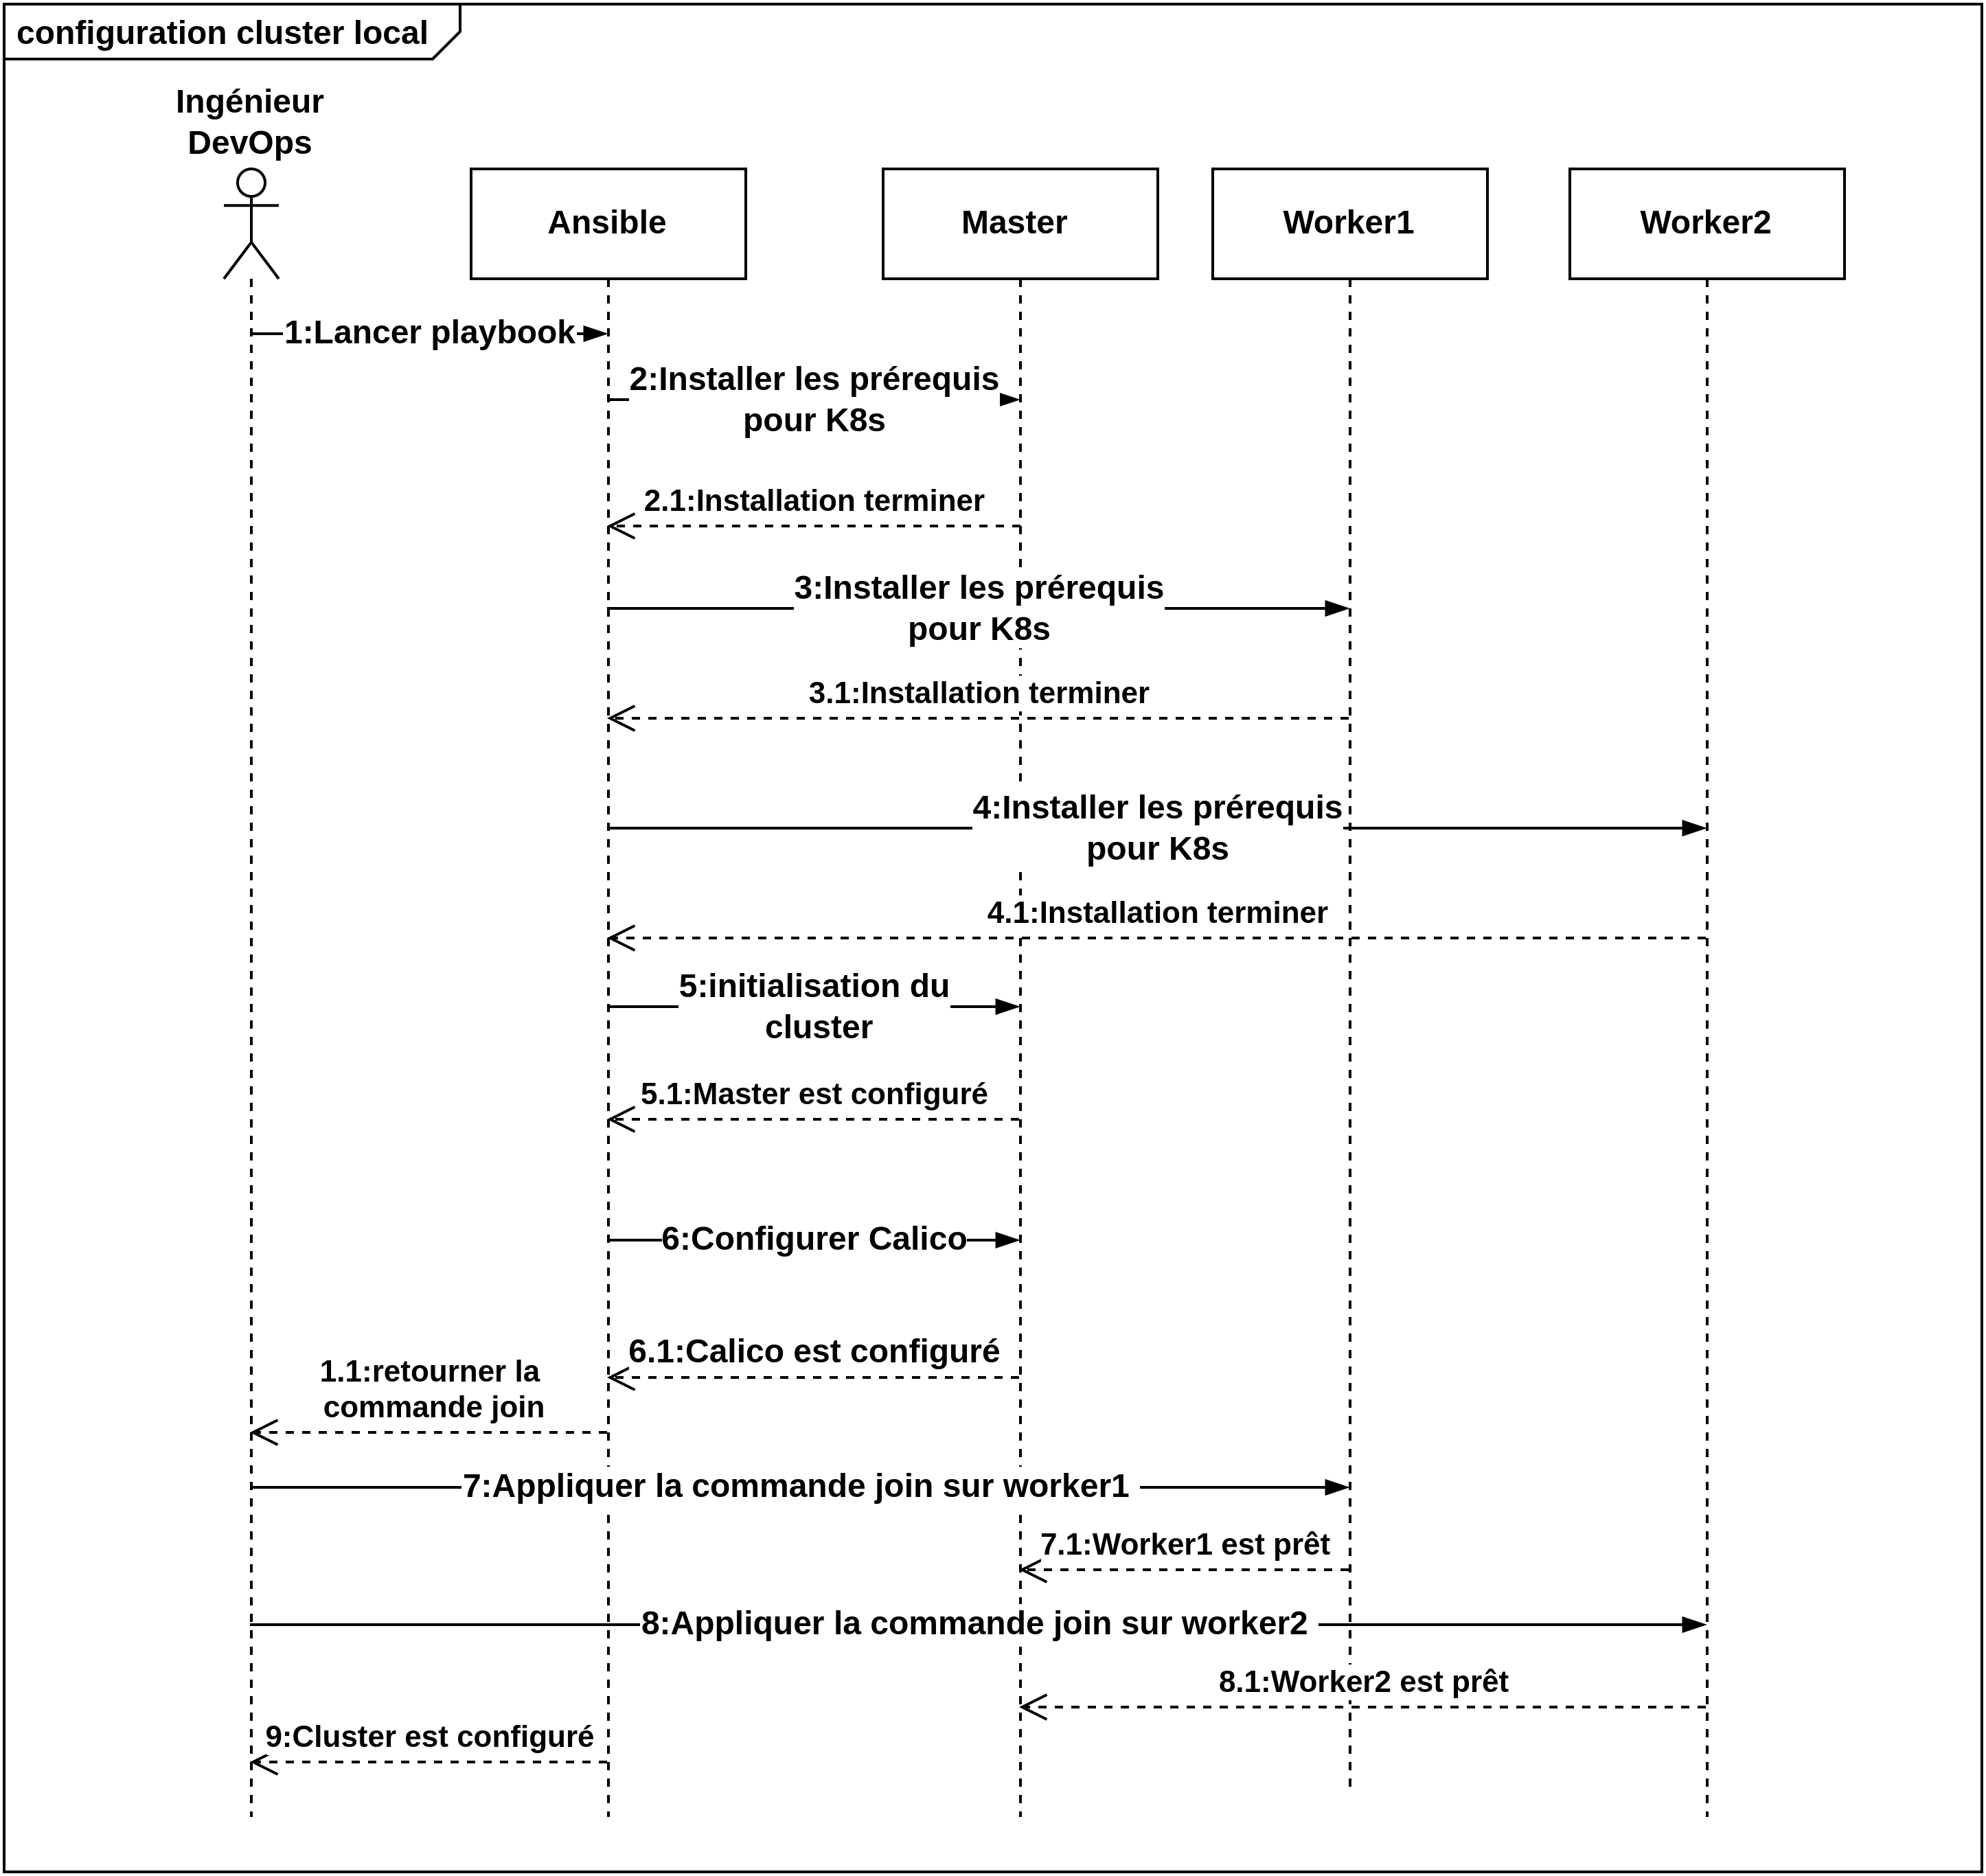
\includegraphics[height=15cm,width=18cm]{SEQCLUSTER.png}
                    \end{center}
                    \caption{Diagramme de séquence « Configuration de cluster local »}
                    %\floatfoot{Source: (Citation command)}
                    % avec le package "floatrow"
                    \end{figure}\subsubsection{\fontfamily{ptm}\selectfont\Large Diagramme de séquence « Configuration du pipeline » }
            Nous détaillons ci-dessous les interactions de diagramme de séquence « Configuration du pipeline » (voir figure 3.4)  .
            \begin{figure}[H]
                \begin{center}
                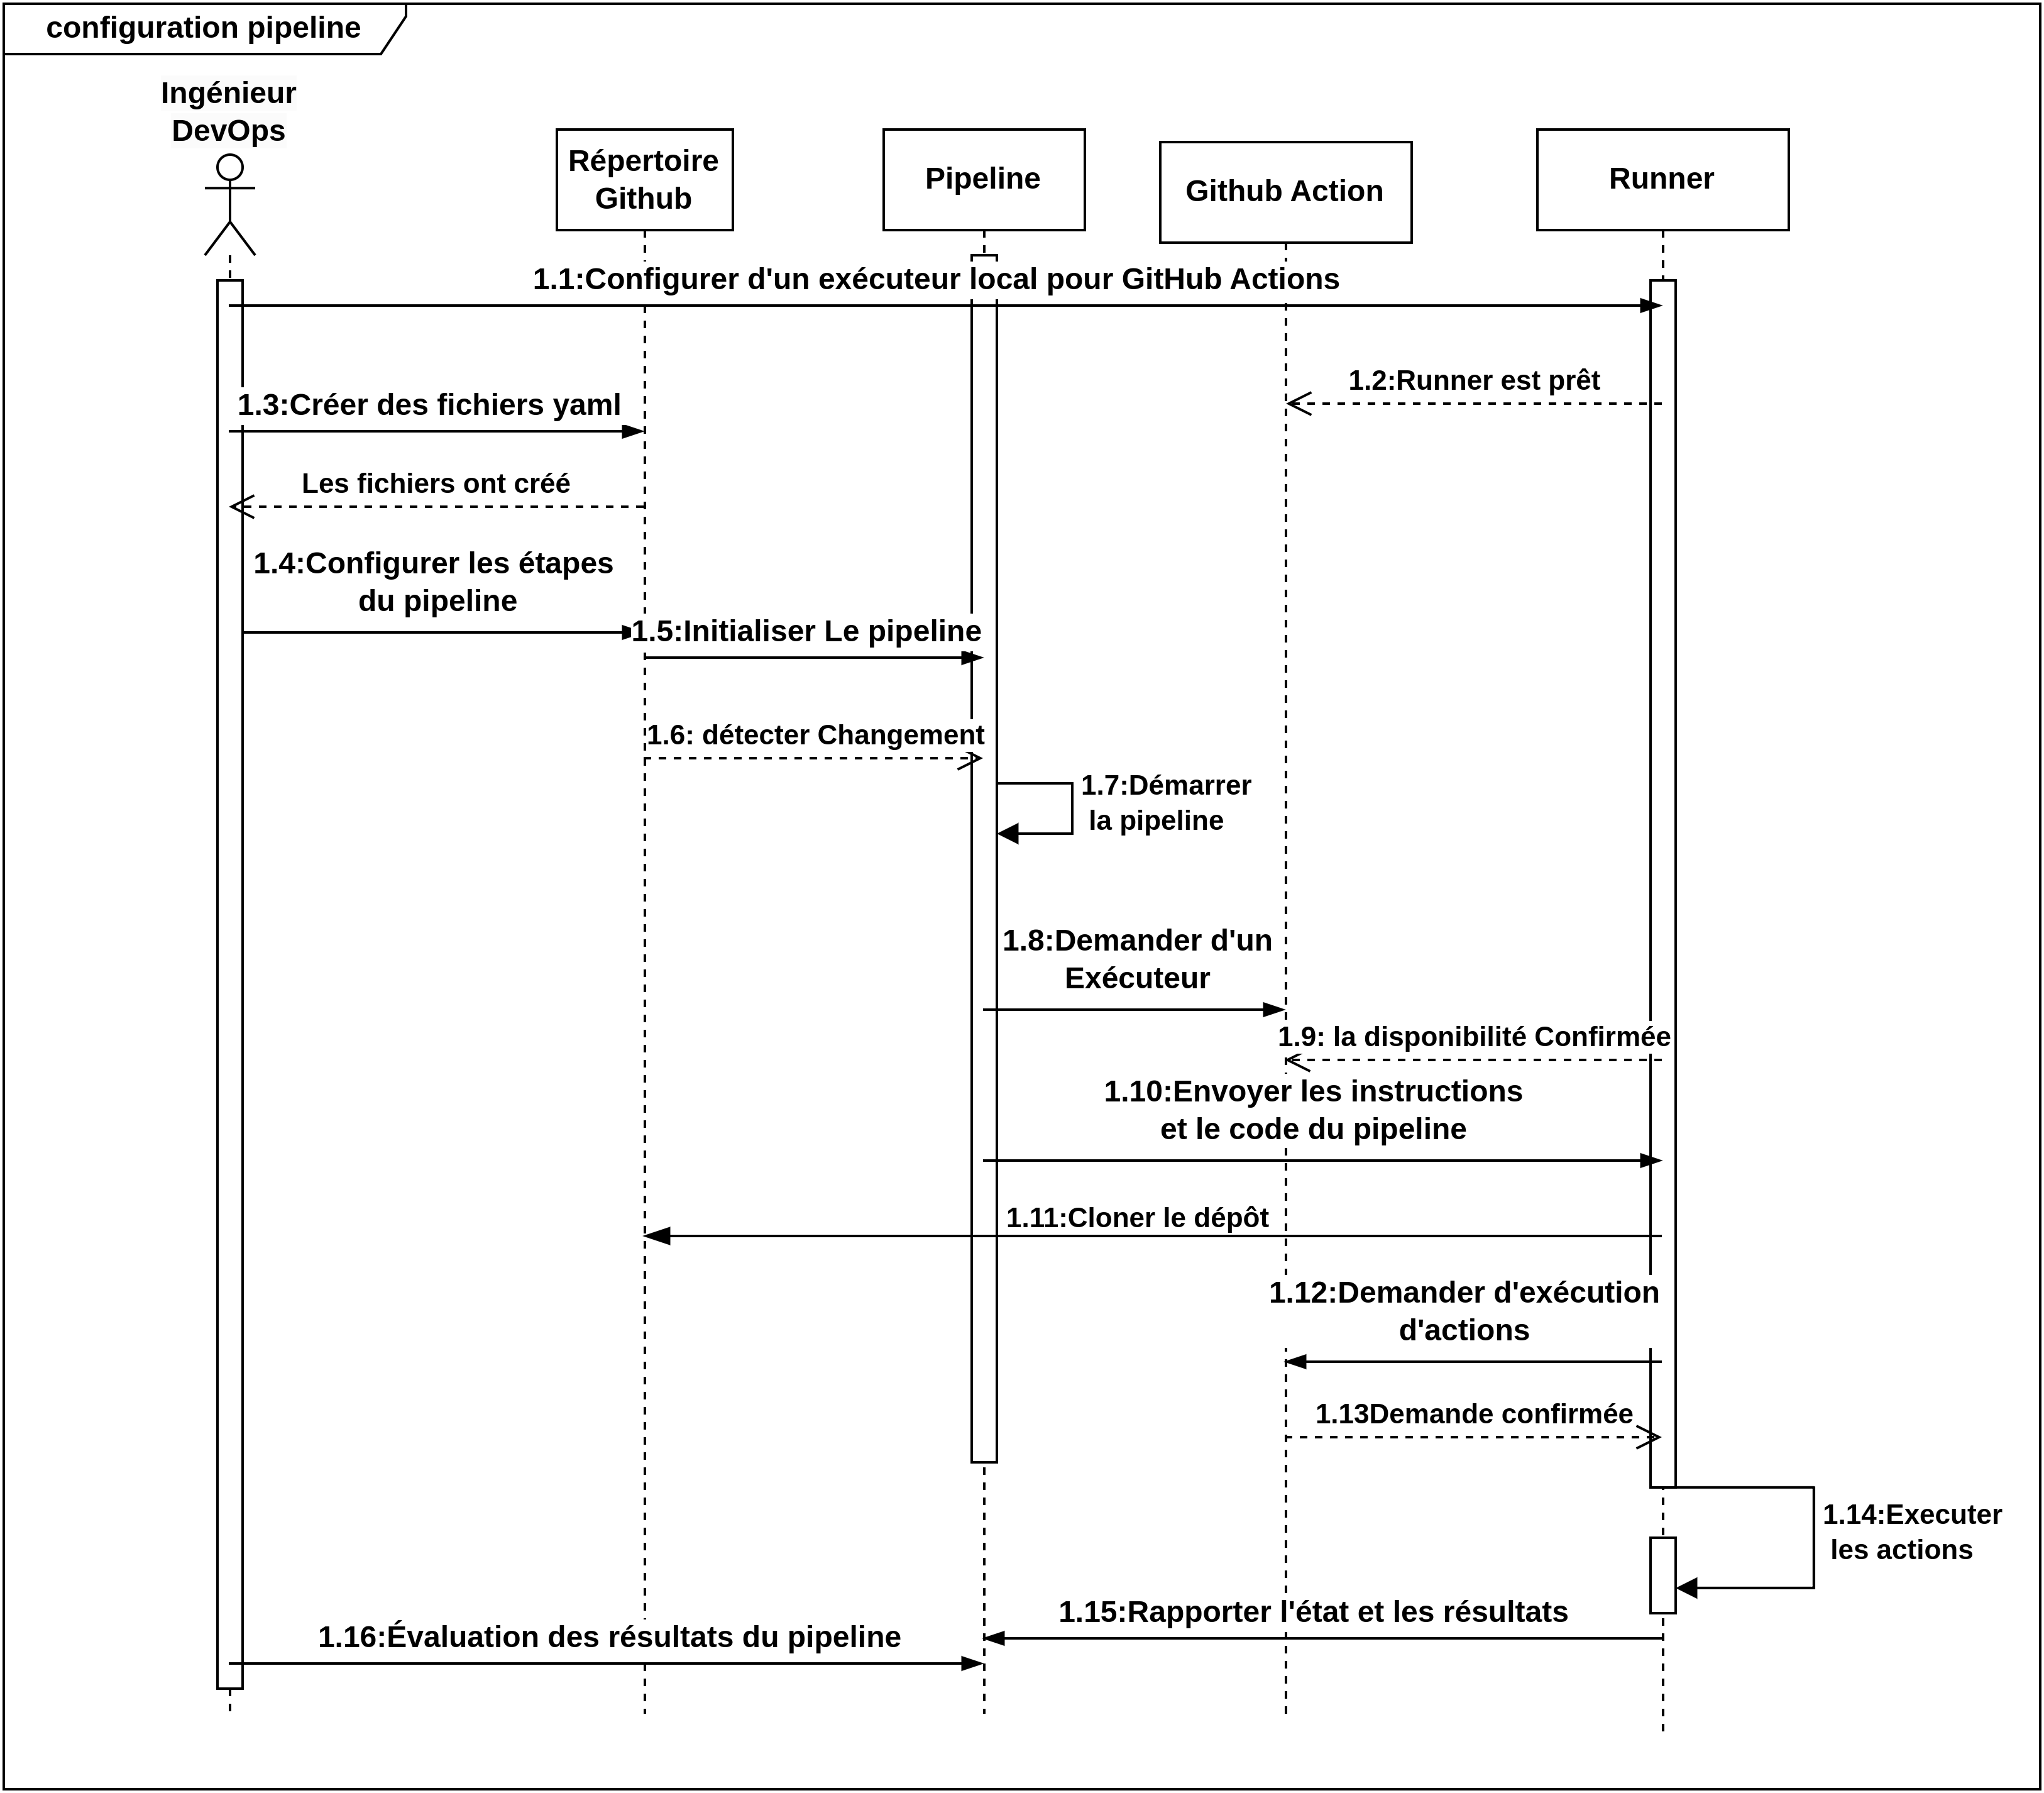
\includegraphics[height=15cm,width=18cm]{SEQPIPELINE.png}
                \end{center}
                \caption{Diagramme de séquence « Configuration du pipeline »}
                %\floatfoot{Source: (Citation command)}
                % avec le package "floatrow"
                \end{figure}
            
\subsection{\fontfamily{ptm}\selectfont\Large Diagramme de classe}
 Le diagramme de classes est un schéma utilisé en génie logiciel pour présenter les classes et les interfaces du système ainsi que leurs relations.La figure ci-dessous représente le 
diagramme de classe de notre travail(voir figure 4.5)\cite{13}.
\begin{figure}[H]
  \begin{center}
  
      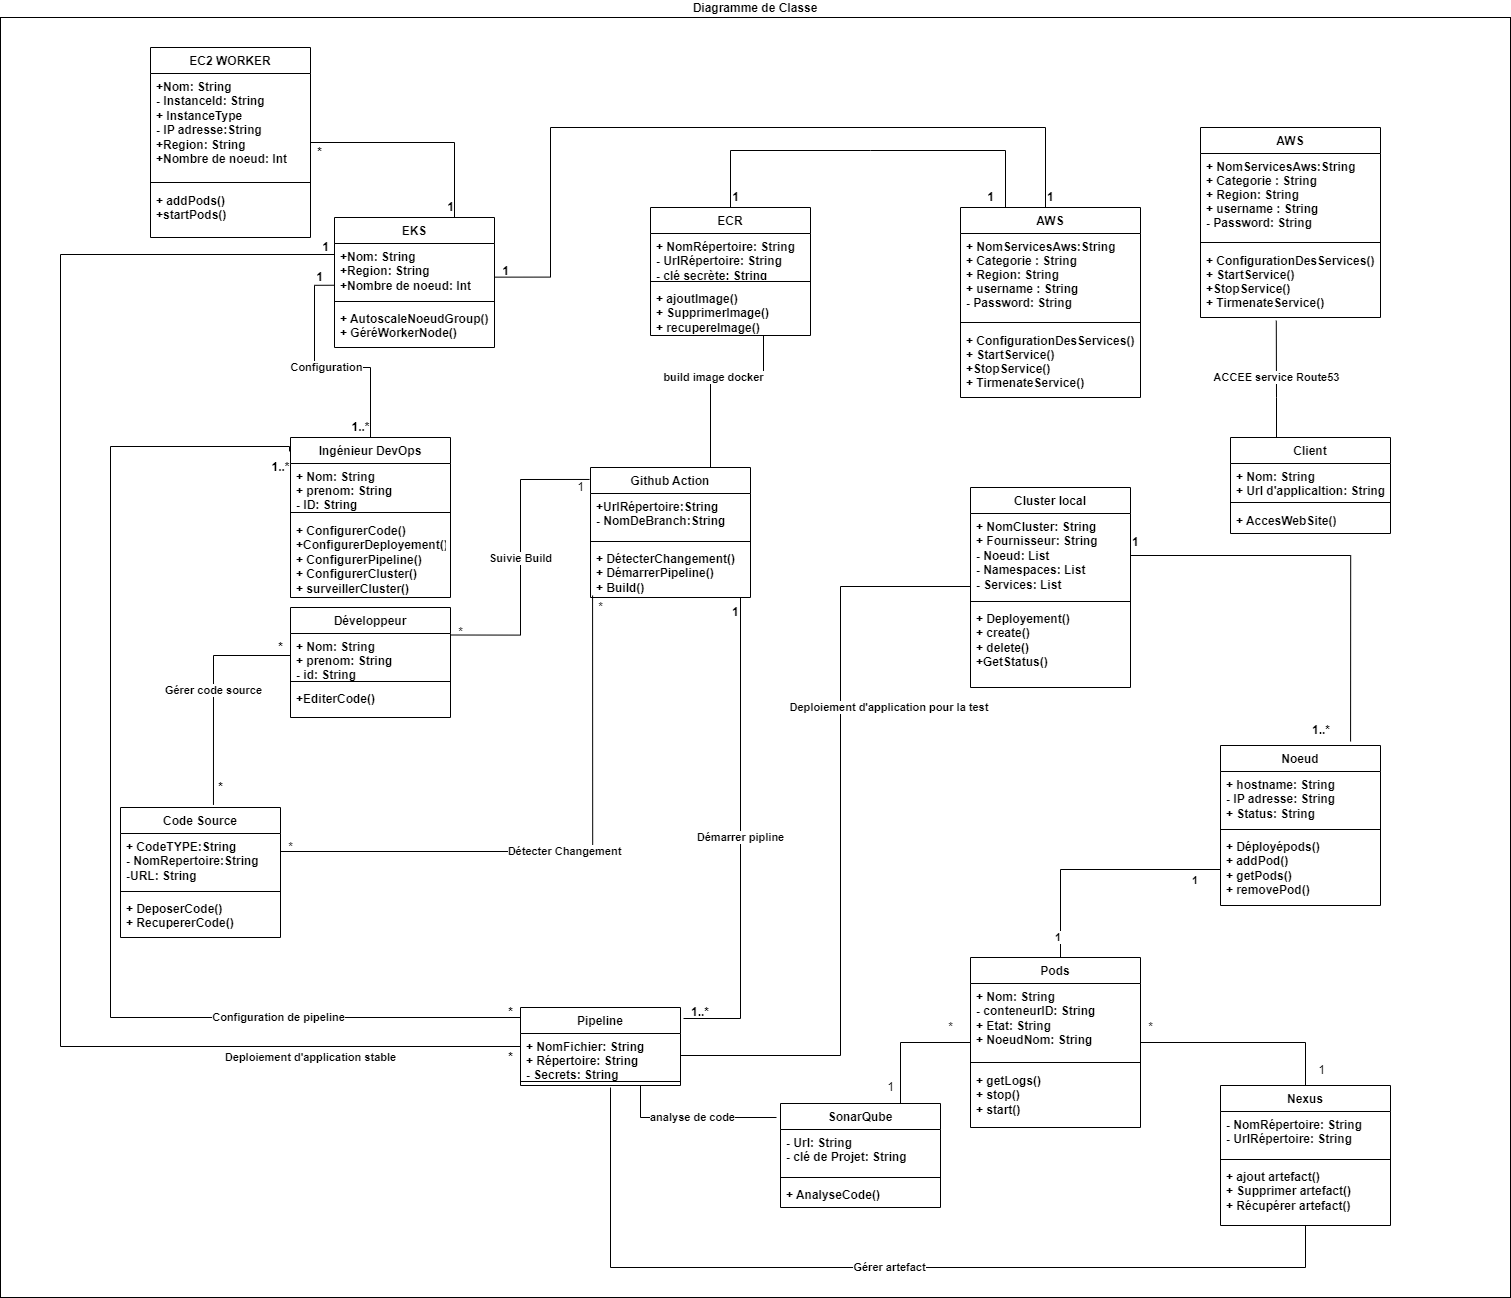
\includegraphics[width=18cm,height=18cm]{ClassDiagram.drawio.png}

  \end{center}
  
  \caption{Diagramme de classe global}
\end{figure}
\subsection{\fontfamily{ptm}\selectfont\Large Diagramme de déploiement}
 Un diagramme de déploiement est une vue statique qui sert à représenter l'utilisation de l'infrastructure physique par le système et la manière dont les composants du système sont répartis ainsi que leurs relations entre eux (voir figure 4.6)\cite{15}.
\begin{figure}[H]
  \begin{center}
  
    \fbox{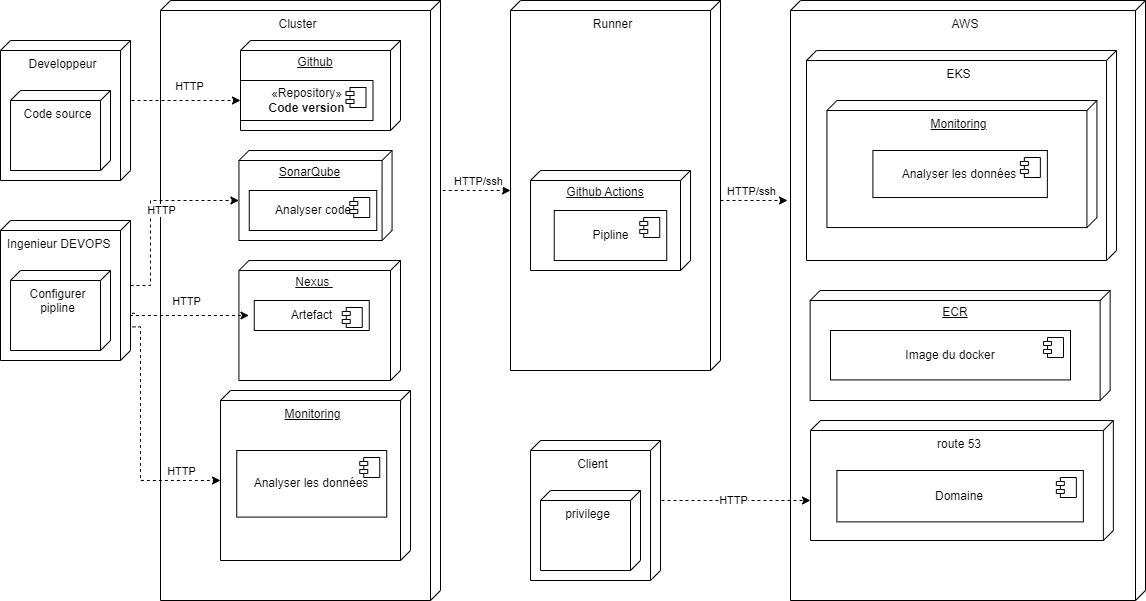
\includegraphics[height=18cm,width=18cm]{deploiment-1.drawio.png}}

  \end{center}
  
  \caption{Diagramme de déploiement global}
\end{figure}
\section{\fontfamily{ptm}\selectfont\Large Méthodologie de conception}
Il est indispensable de choisir une méthodologie de développement  et nous avons choisir la méthodologie (CI/CD). \\
L’Intégration Continue (CI) et la Livraison Continue (CD) regroupent un ensemble de principes et de pratiques permettant aux équipes de développement d’apporter des changements au code informatique de façon plus fiable et plus fréquente.\\
L’implémentation du CI/CD est au coeur des méthodologies de développement agile et DevOps. Elle permet aux équipes de développement logiciel de se focaliser sur les besoins de l’entreprise, la qualité du code et la cybersécurité. Les étapes de déploiement sont automatisées.Ainsi , les pipelines CI/CD permettent aux entreprises d’améliorer fréquemment leurs applications tout en s’appuyant sur un processus de livraison fiable. La standardisation des builds, les tests, l’automatisation du déploiement laissent les équipes se focaliser sur l’amélioration des applications plutôt que sur des détails techniques.\\
Cette pratique est idéale pour la méthode DevOps, car elle évite un mauvais alignement entre des développeurs désirant pousser le code trop fréquemment et les équipes ops en quête de stabilité des applications. L’automatisation permet de pousser des changements de code plus fréquemment, tandis que les configurations standardisées et le testing continu améliorent la stabilité\cite{20}(Voir figure 4.7).\\[0.1cm]
\begin{figure}[H]
  \begin{center}
  
      \fbox{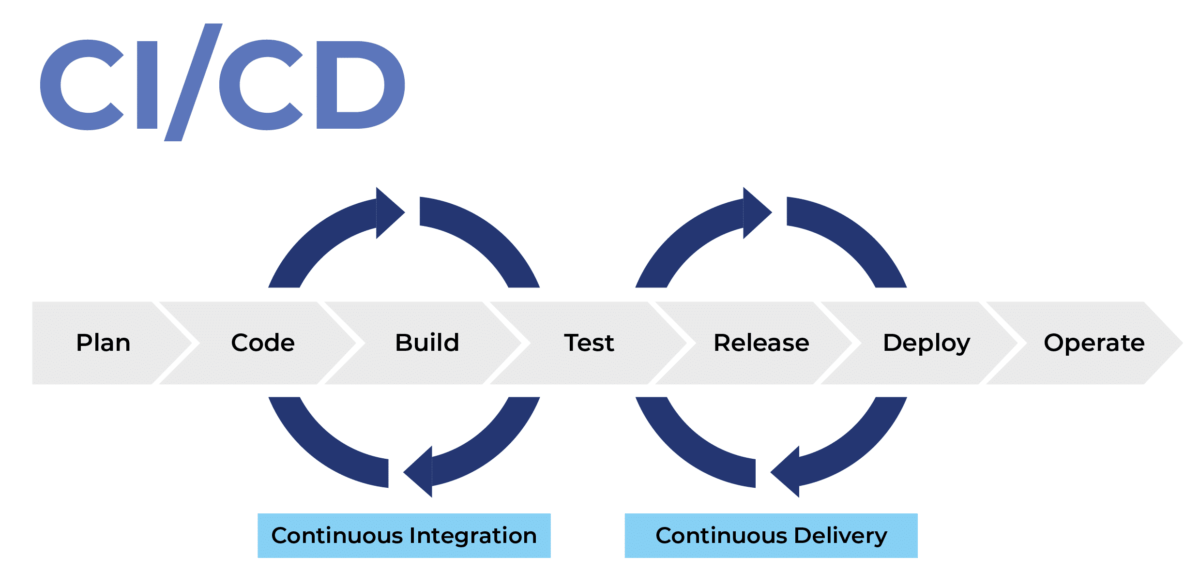
\includegraphics[height=11cm,width=15cm]{besoins/CI-CD-fonctionnement.png}}

  \end{center}
  
  \caption{Méthodologie de développement CI/CD}
\end{figure}
\section{\fontfamily{ptm}\selectfont\Large Architecture technologique de la solution}

 Pour plus de clarté, nous allons diviser notre architecture globale en deux parties.\\
\indent--Partie locale: \\[0.02cm]
La figure (figure: 2.15) représente les ressources utiliser localement dans le projet.


\begin{figure}[H]
\centering
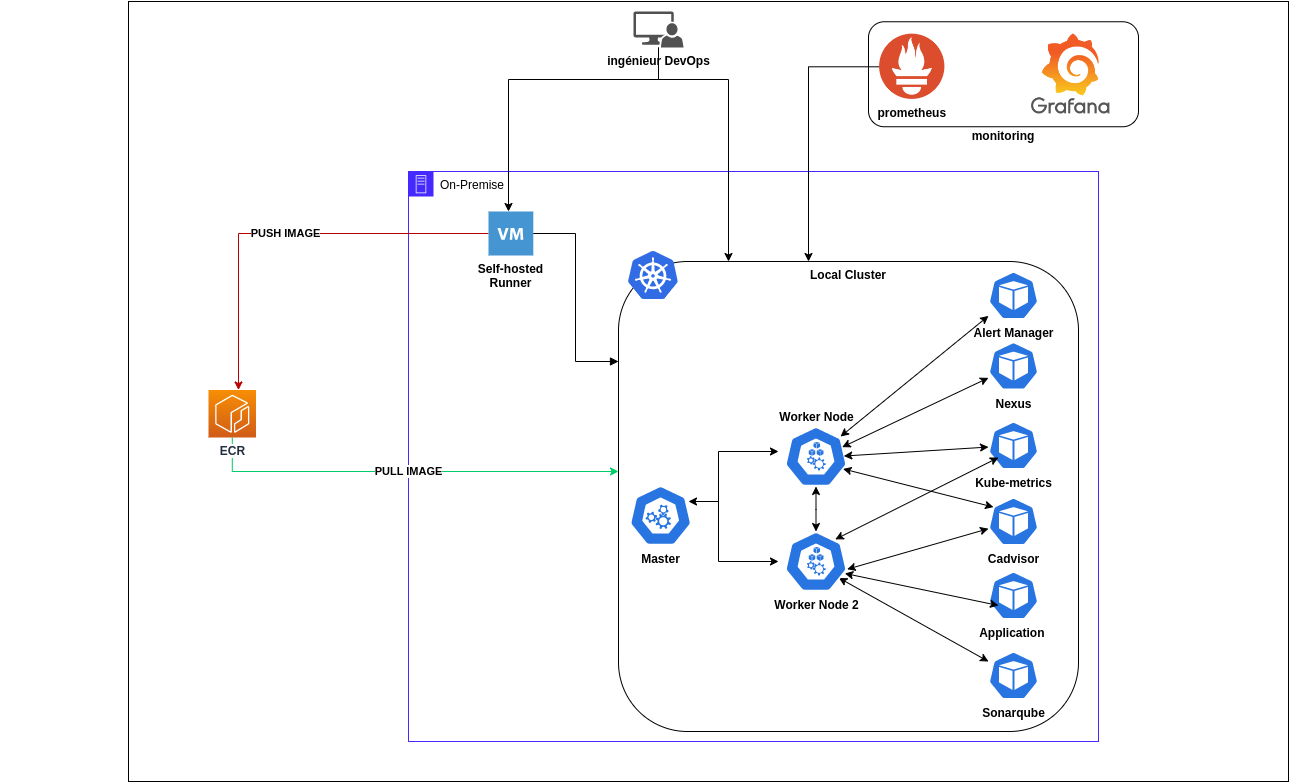
\includegraphics[width=15cm,height=12.5cm]{LOCAL.drawio.png}

  \caption{Partie local}
\end{figure}


\begin{tikzpicture}
  \draw[fill=black] (2,2) circle (2pt);
\end{tikzpicture} 
 Le cluster local dans l’architecture globale fonctionne comme un environnement dédié pour les tests et le développement. Il est configuré et géré par l'ingénieur devops, qui dispose des droits et des permissions nécessaires. Le cluster local est composé de plusieurs composants clés qui facilitent le développement efficace et tester les flux de travail.     \\[0.02cm]
 \indent
 
\begin{tikzpicture}
  \draw[fill=black] (2,2) circle (2pt);
\end{tikzpicture} 
 Dans le cluster local, plusieurs nœuds ou machines virtuelles sont fournies pour créer un environnement similaire à la configuration de production. Ces nœuds exécutent des conteneurs ou d’autres outils de test, permettant la possibilité de simuler le comportement et les performances de l’environnement de production localement. L’ingénieur DevOps supervise la configuration et la gestion du cluster local, en assurant sa disponibilité et sa stabilité pour les activités de test et de développement.\\[0.02cm]
 \indent
 
\begin{tikzpicture}
  \draw[fill=black] (2,2) circle (2pt);
\end{tikzpicture} 
 Pour surveiller le cluster local, l’ingénieur devops déploie Grafana et Prometheus, qui fournissent des informations précieuses sur les performances et la santé du cluster. Ces outils de surveillance permettent de suivre l’utilisation des ressources, de détecter et de résoudre les problèmes rapidement, ce qui permet l’amélioration continue et l’optimisation de l’environnement de test local.\\[0.02cm]
 \indent
 
\begin{tikzpicture}
  \draw[fill=black] (2,2) circle (2pt);
\end{tikzpicture}
 L’ingénieur devops configure également un exécuteur local pour GitHub Actions. Cet exécuteur permet de déclencher des pipelines. Dans le cas de la branche principale, un pipeline démarre et les actions de déploiement nécessaires sont exécutées sur le cluster local. Cela permet l'ingénieur devops de valider les changements dans un environnement qui ressemble beaucoup à la configuration de production, assurant robustesse et fiabilité.
 \\[0.02cm]
 \indent
 
\begin{tikzpicture}
  \draw[fill=black] (2,2) circle (2pt);
\end{tikzpicture}
L’ingénieur de devops configure l’environnement pour extraire les images de conteneurs d’un dépôt ECR privé, qui stocker et gérer les images de conteneurs. Les images du dépôt sont séparées par des versions telles que 1.0.0 , 0.0.1 pour les tests.
 
 
\indent{\fontfamily{ptm}\selectfont\scalefont{1.3}--Partie AWS:} \\
La figure ci-dessous représente les ressources cloud utilisés dans notre projet.
\begin{figure}[H]


  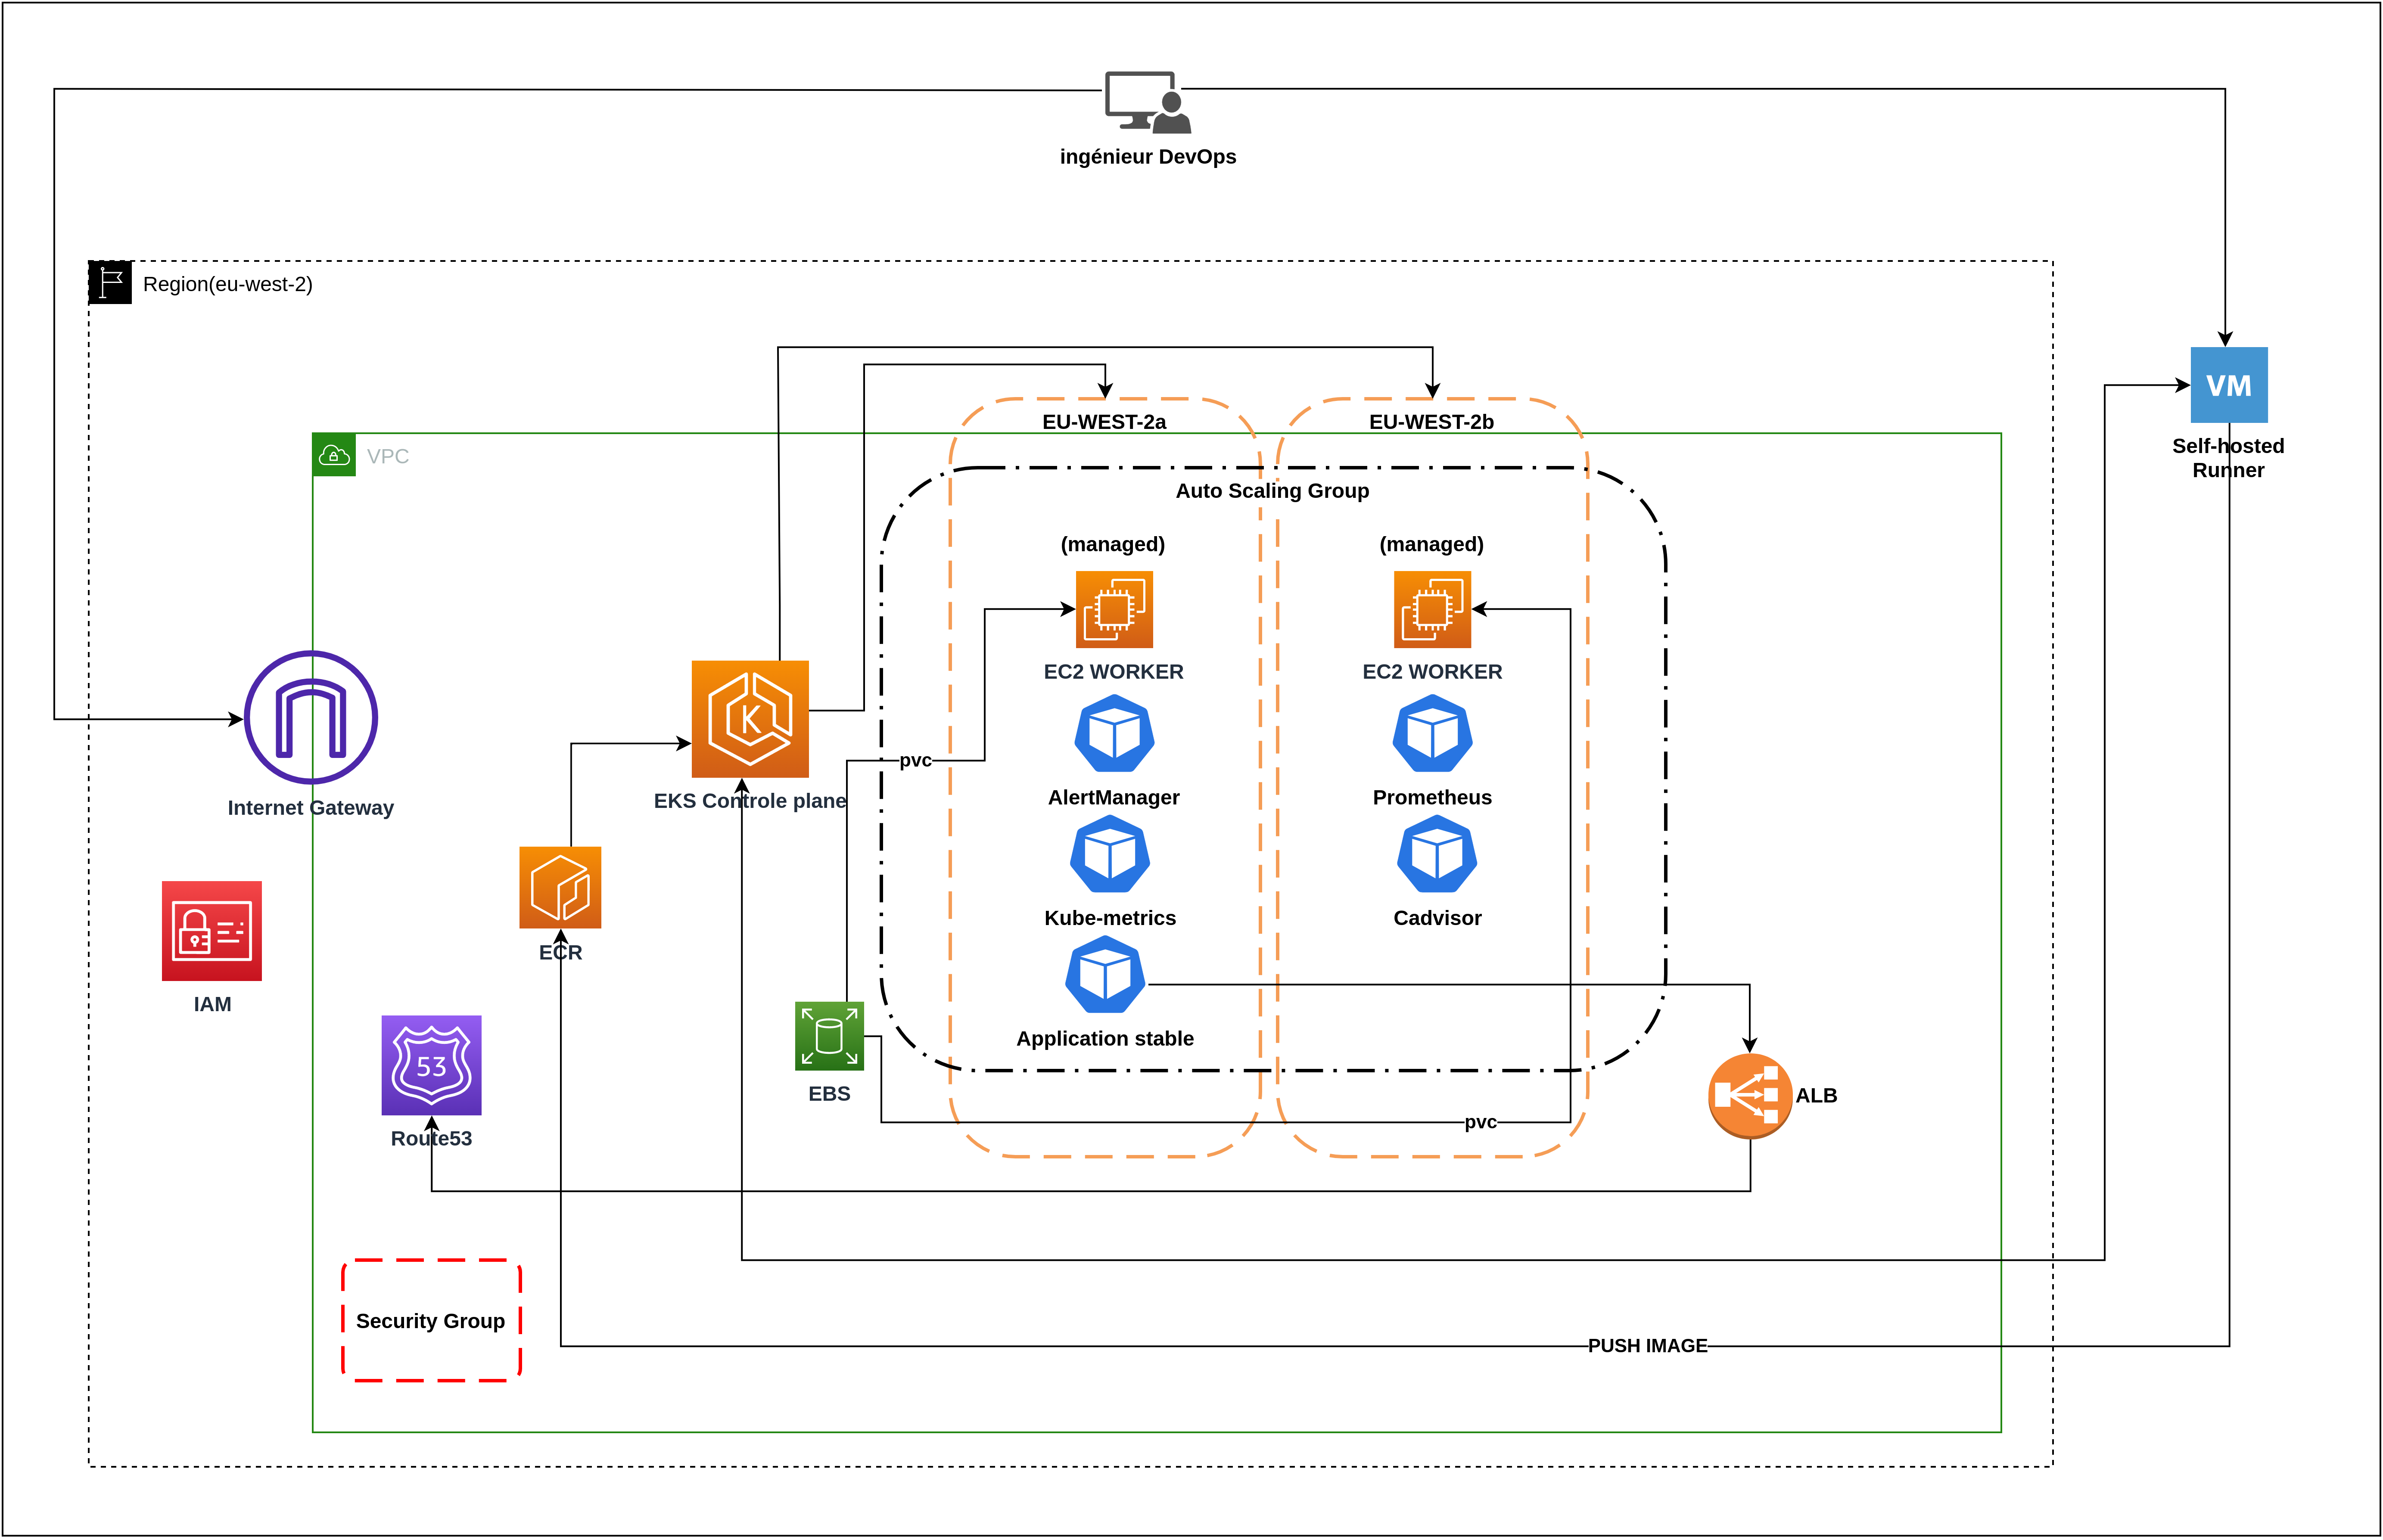
\includegraphics[width=18cm,height=14cm]{PARTIEEKS.drawio.png}
  
    \caption{Partie AWS}
  \end{figure}
  \indent
  
\begin{tikzpicture}
   \draw[fill=black] (2,2) circle (2pt);
 \end{tikzpicture}
 Le cluster EKS se compose de nœuds de travail, qui sont des instances EC2 qui exécutent les conteneurs contenant la charge de travail de l’application. L’ingénieur DevOps assure l’approvisionnement et la mise à l’échelle appropriés des nœuds de travailleurs en fonction des exigences de l’application et de la charge de travail. Cela implique de configurer des politiques de mise à l’échelle automatique pour ajuster automatiquement le nombre de nœuds de travail afin de gérer efficacement les différents charges de travail.
 \\[0.01cm]
 \indent
 
\begin{tikzpicture}
  \draw[fill=black] (2,2) circle (2pt);
\end{tikzpicture}
Pour gérer le trafic entrant et le distribuer à travers les conteneurs du cluster EKS, un Load balancer est lancé pour aider à atteindre une haute disponibilité et une tolérance aux pannes en transférer les demandes vers les conteneurs, assurant ainsi une performance et une fiabilité optimales de l’application.
\\[0.01cm]
\indent

\begin{tikzpicture}
 \draw[fill=black] (2,2) circle (2pt);
\end{tikzpicture}  
Lorsque la branche EKS est déclenchée par des développeurs  leur code source, un pipeline dédié est lancé. Pour exécuter les actions de déploiement nécessaires sur le cluster EKS, un exécuteur configuré par l’ingénieur devops utilise son contexte et ses autorisations pour intéragir efficacement avec le cluster. Cela permet un déploiement continu de l’application dans l’environnement de production hébergé sur le cluster EKS.
\\[0.01cm]
\indent

\begin{tikzpicture}
 \draw[fill=black] (2,2) circle (2pt);
\end{tikzpicture}  
La surveillance du cluster EKS est également une responsabilité de l’ingénieur DevOps. Une fois Prometheus installé sur EKS, il fournit des informations complètes sur les performances, l’utilisation des ressources et les paramètres de santé du cluster. Cet outil permet à l’ingénieur de détecter et de résoudre rapidement les problèmes potentiels, assurant le bon fonctionnement de l’environnement de production.\\[0.3cm]
          
\textbf{\huge Conclusion}\\[0.5cm] 

Dans ce chapitre nous avons décrit les différents besoins fonctionnels et non fonctionnels. Aussi, nous avons décrit les différents acteurs du système. Puis nous avons présentée les "User stories" en forme d'un product backlog. Par la suite, nous avons illustré les cas d'utilisation avec des diagrammes. Puis, nous avons décrit les différents diagrammes de conception. Aussi, nous avons décrit la méthode de conception utilisée dans notre projet. Enfin, nous avons présenté l'architecture globale qui expliquera le fonctionnement du projet. Dans le chapitre suivant nous passerons à la phase de réalisation du projet.

